\subsection{Radar Simulations} \label{compvis_radarsims}

    \subsubsection{Introduction and Physical Principles} \label{rory_radar_principles}
    
        As outlined in Section \ref{simulation_justification}, the limited diversity of the radar dataset necessitates physics-driven simulations to replicate the noise and clutter encountered in real-world environments. These simulations aim to validate the CNN’s robustness to physical processes that degrade B-scan clarity, ensuring reliable performance under operational conditions.
    
        The electromagnetic phenomena governing radar losses are:
        \begin{itemize}
        
            \item \textbf{Antenna losses}: Mismatch losses (approximately −1 dB \cite{daniels2005gpr}), and efficiency losses (excluded as secondary to subsurface effects).
            
            \item \textbf{Transmission losses}: Signal attenuation from reflections at air-soil and soil-air interfaces.
            
            \item \textbf{Material losses}: Frequency-dependent attenuation within heterogeneous soils.
            
            \item \textbf{Scattering losses}: Arising from subsurface inhomogeneities in soil composition, and soil surface roughness.
        
        \end{itemize}
        
        To model these effects, finite-difference time-domain (FDTD) simulations were conducted using \textit{gprMax} \cite{warren2016gprmax}, an open-source framework for solving Maxwell’s equations in 3D geophysical media. This approach captures full-wave electromagnetic behaviour, including wave propagation, reflection, and attenuation, while explicitly accounting for soil heterogeneity. The inclusion of surface roughness is not considered in this report, as for the purposes of validating the CNN-driven detection framework, modelling of subsurface heterogeneity suffices to ensure robustness to clutter. This is however a significant contribution to the clutter observed in an operational GPSAR system, and future work should consider this aspect that has been overlooked here.
     
    
    
    \subsubsection{gprMax Implementation}

        \paragraph{Radar}
        
             The source/receiver configuration follows recommendations provided by Huirui (see Section XX) and employs a Ricker waveform as the excitation signal. The Ricker waveform is widely used in GPR and seismic applications for its clear central frequency and well‐defined bandwidth properties \cite{dummyRef2}. A central frequency of 1.5\,GHz was chosen, as it provides a good compromise between penetration depth and resolution—even in moderately moist soils where deeper penetration is required. The transmitter and receiver are modelled as Herzian dipole antennas, which represent the electromagnetic field distribution in practical GPR systems \cite{dummyRef3}.
    
        \paragraph{Domain}

            The simulated computational domain spans $0.8\times 0.3\times0.02$\,m ($x\times y\times z$), representing a quasi-2D space. The domain is discretised into cubic elements of side length 0.002\,m , 100 times smaller than the wavelength of the radar pulse. Two thirds of the domain is occupied with soil, and the rest with air. A circular landmine with radius 5\,cm was buried with its centre 0.1\,m below the surface of the soil, and was modelled as a perfect electric conductor (PEC), representative of a metallic landmine.


        \paragraph{Boundary Conditions}
        
            Perfectly matched layers (PMLs) are used as obsorbing boundary conditions on all sides of the domain, to mimick an open boundary. The source and receiver were placed more than 20 cells away from the PML regions to avoid erroneous interference. Each simulation was run for 5$\times$10$^{\text{-9}}$\,s, enough to capture all the relevant electromagnetic phenomena.

        
    
    \subsubsection{Heterogeneous Soil Model}
    
        A realistic simulation of electromagnetic wave propagation necessitates an accurate representation of the subsurface. In this work, the heterogeneous soil is modelled using the Peplinski model, which characterises soil dielectric properties based on sand fraction, clay fraction, bulk density, sand-particle density and volumetric water fraction range, over a frequency range of 1-18\,GHz. To capture the natural spatial variability, a fractal generation technique is employed \cite{dummyRef5}. This method replicates the self-similar patterns observed in natural soils over multiple scales, thereby enhancing the fidelity of the simulation, and accurately accounting for the heterogeneity in the soil. Detail of the Peplinski soil model, and the fractal generation technique can be found in \cite{warren2016gprmax}. 

        \paragraph{Soil Parameters}

            For the simulation to give realistic results, it is initialised with accurate soil parameters for Ukraine. Ukraine is mostly covered with the very fertile Chernozem soil \footnote{\url{https://www.britannica.com/place/Ukraine/Soils}}, the properties of which were taken from \cite{suleymanov2021chernozem}, and are summarised here.

            \begin{table}[htbp]
              \centering
              \caption{Properties of Chernozem Soils}
              \begin{tabular}{@{} l l @{}} 
                \toprule
                \textbf{Property} & \textbf{Value} \\
                \midrule
                Clay fraction & $\sim 30\%$ \\
                Sand fraction & $\sim 70\%$ \\
                Bulk density & $\sim 1.4$ g/cm$^3$ \\
                Sand particle density & $2.65$ g/cm$^3$ \\
                Volumetric water fraction range & $1\% - 10\%$ \\
                \bottomrule
              \end{tabular}
            \end{table}
    
        \begin{figure}[htbp]
            \centering
            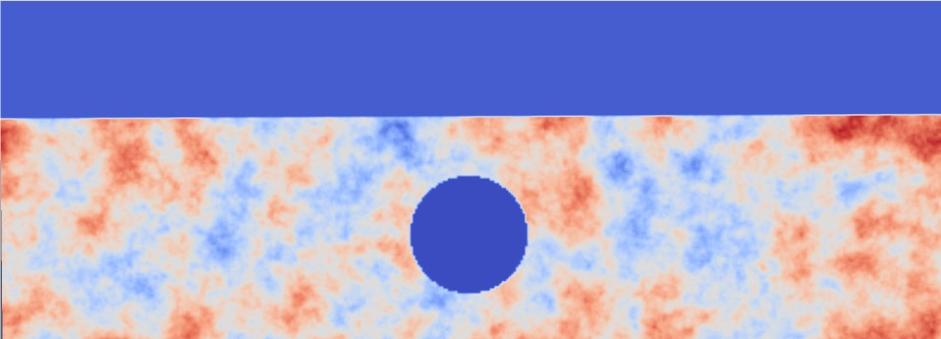
\includegraphics[width=0.8\textwidth]{figs/Rory/radar_domain.pdf}
            \caption{Simulation domain viewed in ParaView.}
            \label{fig:radar_domain}
        \end{figure}
        \footnote{\url{https://www.paraview.org/}}
    
    \subsubsection{Results and Validation}
    
        Figure~\ref{fig:radar_results} shows the simulated radar responses, illustrating the backscattered signatures generated by the presence of a buried landmine. These responses have been compared with real GPR data obtained from controlled field experiments \cite{dummyRef7}, demonstrating reasonable agreement. However, computational limitations restrict the number of simulations that can be feasibly run, and the current model assumes a simplified environment with flat ground, no foliage, and an absence of puddles or other surface irregularities. These factors may contribute to discrepancies between simulated and real-world data.
    
        \begin{figure}[htbp]
            \centering
            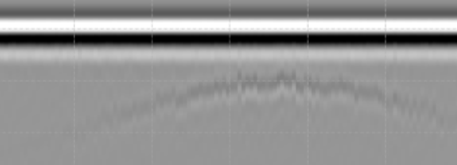
\includegraphics[width=0.8\textwidth]{figs/Rory/sim_bscan_cropped.png}
            \caption{Raw simulated B-scan (no digital enhancement)}
            \label{fig:original_bscan}
        \end{figure}
    
    \subsubsection{Data Augmentation}
    
        Running these simulations is expensive, so one should make the most of each simulation performed. From this one simulation, multiple image augmentations were applied, each representing a physical process. The transforms considered were stretching, cropping and adding Gaussian blur, and combinations of the above. When this is done to our simulated Bscan, we generate a dataset of 90 images. This is enough to test whether our pre-trained CNN is robust to heterogeneous soil properties.
        \begin{figure}[htbp]
            \centering
            
            % First subfigure
            \begin{subfigure}[b]{0.32\textwidth}
                \centering
                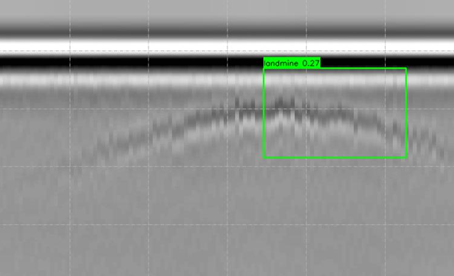
\includegraphics[width=\textwidth]{figs/Rory/sim_bscan_clahe_detection_cropped.png}
                \caption{Simulated B-scan with CLAHE applied. Bounding boxes visible.}
                \label{fig:bscan_clahe}
            \end{subfigure}
            \hfill
            % Second subfigure
            \begin{subfigure}[b]{0.32\textwidth}
                \centering
                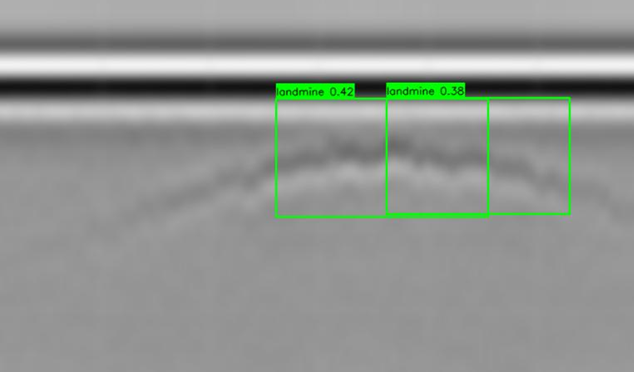
\includegraphics[width=\textwidth]{figs/Rory/sim_bscan_clahe_detection_blur_cropped.png}
                \caption{Simulated B-scan with CLAHE and Gaussian blur. Bounding boxes visible.}
                \label{fig:bscan_blur}
            \end{subfigure}
            \hfill
            % Third subfigure
            \begin{subfigure}[b]{0.32\textwidth}
                \centering
                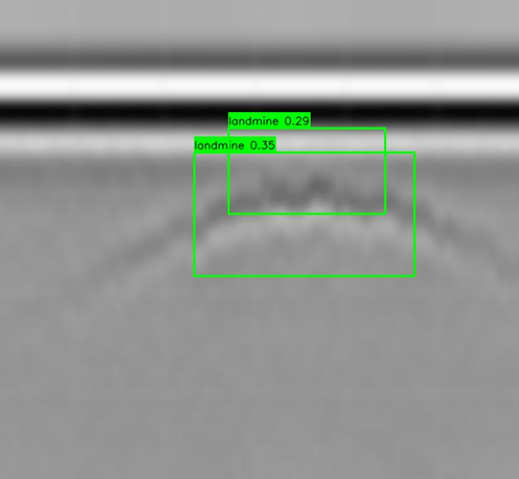
\includegraphics[width=\textwidth]{figs/Rory/sim_bscan_clahe_detection_blur_stretched_cropped.png}
                \caption{Simulated B-scan with CLAHE, Gaussian blur, and stretching. Bounding boxes visible.}
                \label{fig:bscan_blur_stretched}
            \end{subfigure}
            
            \caption{Comparison of simulated B-scans under different pre-processing steps (CLAHE, Gaussian blur, stretching). Each image shows bounding boxes around detected targets.}
            \label{fig:sim_bscan_comparison}
        \end{figure}
        
    
    \subsubsection{CV Results}
    
        The augmented radar data were subsequently analysed using the pre-trained CNN (SECTION XX) to evaluate its efficacy in detecting buried landmines. Precision and recall metrics were calculated on the augmented dataset, with the results (summarised in Table~\ref{tab:cv_results}) indicating that the combined approach of GPSAR and advanced CV techniques is promising for practical landmine detection. In particular it is noted that we can achieve a high precision with moderate recall with the GPSAR sensor, and that the CNN, although trained on a very homogenous 'clean' dataset generalised well to a more varied dataset from high-order simulations that directly model the noise processes (which we have argued in SEC XX is very important).
        
        In summary, our results indicate that a GPSAR sensor combined with a CNN detection algorithm—developed entirely using free and open-source software—holds considerable promise for robust detection of buried landmines across a range of environments. The system's demonstrated ability to generalize to complex simulated noise suggests resilience under real-world conditions, and we believe that the current performance likely represents a conservative lower bound. With further training and additional data, significant improvements in detection accuracy are achievable, offering a highly maintainable and effective solution, that can improve as more context specific data becomes available.